% -*- mode: LaTeX; coding: utf-8; -*-

\chapter{Analyysi}

Tässä luvussa käydään vaiheittain läpi yhden valitun palvelun analysointi sekä esitetään perustelut, joiden pohjalta tehtyihin ratkaisuihin on päädytty. 
Luvussa myös esitellään analysoinnista saatuja tuloksia, sekä pohditaan näihin johtaneita syitä. Lopuksi vielä esitetään jatkotutkimuksen kannalta 
tärkeitä kehitysideoita, joita syntyi tutkimuksen aikana. 
 
\section{Tutkimuksen toteutus}

Saamamme materiaali koostui neljästä eri Web-palvelusta, joista analyysiin valitsimme yhden. Muista palveluista saadut lokitiedostot käsiteltiin
myös valmiiksi, mutta koska lokitietoja oli määrällisesti niin paljon, päädyimme tarkastelemaan tarkemmin vain yhtä. Valitsemastamme palvelusta
analysoimme myös vain viikon mittaisen jakson. Tähän ratkaisuun päädyttiin sen takia, että analysoitavaa dataa oli kerätty noin puolen vuoden ajalta,
joten jo yhden palvelun osalta koko datan läpikäymiseen olisi mennyt kohtuuttomasti aikaa. Diffuusikuvausten laskemiseen voitiin
myös käyttää korkeintaan noin 5000 yksittäistä pistettä 2000 pisteen ollessa laskennallisesti vielä tehokasta, koska algoritmin aikavaativuus kasvaa
eksponentiaalisesti verrattaessa opetusmateriaalin kokoon. 
 
Esikäsittelyvaiheessa HTTP-kyselyt jaetaan palvelun resurssien mukaan omiin tiedostoihin, joissa ne ovat CVS-formaatissa kuvan ??? mukaisesti. 
Resursseihin kohdistuvat kyselyt vaihtelevat suuresti sen mukaan, kuinka käytetty mikäkin resurssi on. Perinteisen Web-sivuston tapauksessa tähän
vaikuttavat esimerkiksi resurssia käyttävän palvelun käyttöaste ja se, käytetäänkö samaa resurssia useamman sivun osana. 

Analyysissä käyttämämme viikon pituinen jakso sisälsi yhteensä 913 eri resurssia ja näihin kohdistuvat kyselymäärät vaihtelivat muutamasta kappaleesta
aina kymmeniin tuhansiin. Näistä suodatimme pois sellaiset resurssit, joihin kohdistui alle 100 kyselyä ja joiden GET-parametreistä muodostettujen
erilaisten n-grammien määrä oli alle kymmenen. Suodatuksen jälkeen analysoitavaksi jäi 36 resurssia. Käyttämillämme suodatusrajoilla ei ole tekemistä 
itse esikäsittelijän kanssa, vaan suodatusrajat on käyttäjän säädettävissä tiedostosta \texttt{src/InterestingParameters.hs}.
    
Käytetyimmissä resursseissa HTTP-kyselyitä oli kymmeniä tuhansia, joten jokaisesta resurssista ei pystytty suoraan tekemään diffuusiokuvausta johtuen
menetelmän rajoituksista. Ongelma ratkaistiin valitsemalla satunnaisotannalla ilman takaisinpanoa 2000 HTTP-kyselyä niistä resursseista, joissa oli 
kyselyitä yli tämän määrän. Näin ollen jokaisesta resurssista muodostettiin lopulta tiedosto, jossa oli korkeintaan 2000 HTTP-kyselyä.

Analysoitavan palvelun eri resurssit on esitetty kuvassa \ref{service_resources}. Kuvassa vaaka-akselina on käytetty N-grammien lukumäärää ja 
pystyakselina GET-parametrien lukumäärää. Resursseista valitsimme kuusi tarkempaan tarkasteluun, ja ne on merkitty kuvaajaan niiden resurssinumerolla. 
Resurssit pyrimme valitsemaan siten, että jokaisesta ryppäästä olisi yksi valittuna.

\begin{figure}[ht]
\centering
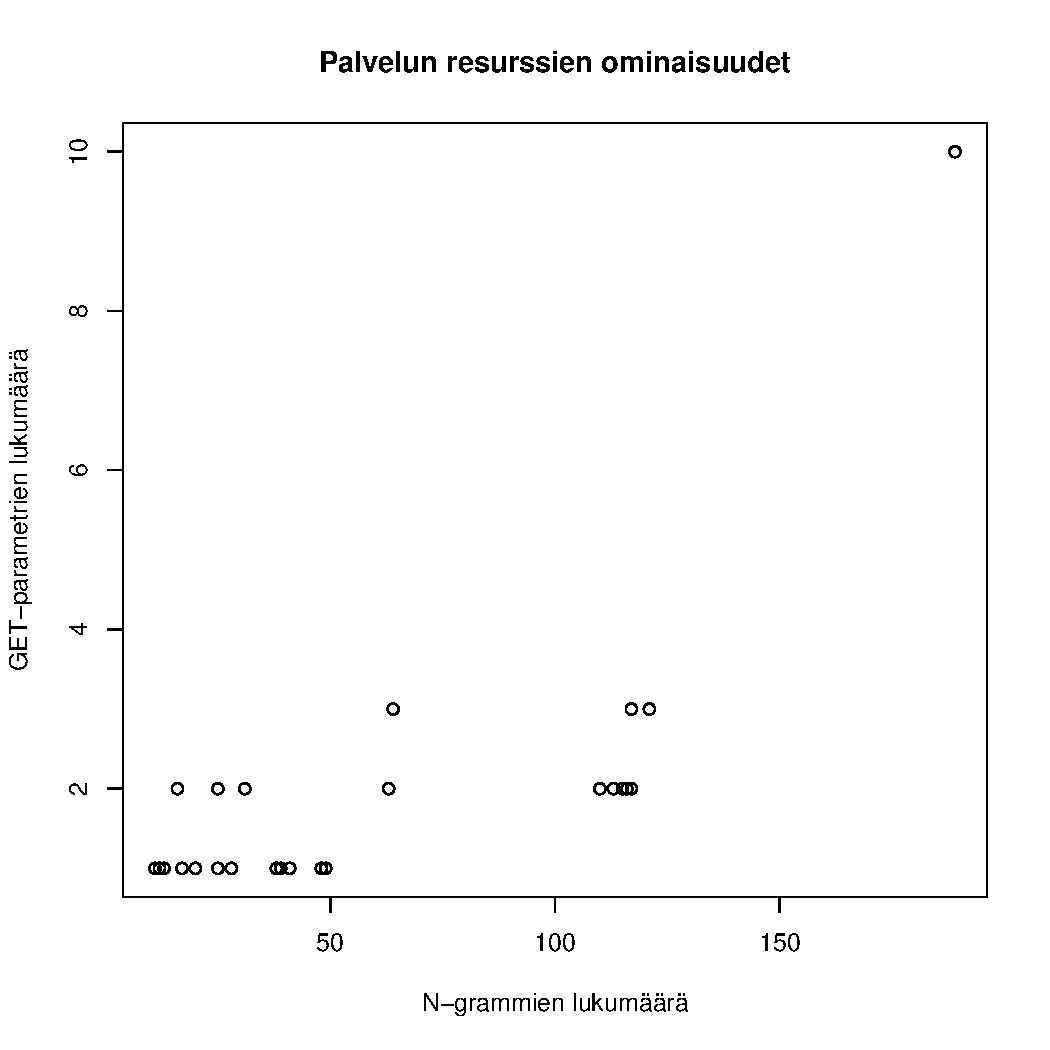
\includegraphics[width=13cm]{pics/service_resources.pdf}
\caption{Palvelun resurssien ominaisuudet.}
\label{service_resources}
\end{figure}

\section{Tulokset}

Palvelun jokaisesta resurssista muodostettiin diffuusiokuvaus käyttäen korkeintaan 2000 pistettä. Näin lasketuista diffuusiokuvauksista muodostettiin
seuraavaksi diffuusiokartta käytäen toista ja kolmatta ominaisvektoria. Esimerkiksi kuvassa \ref{diffusio_1} on resurssin 1 diffuusiokuvauksen pohjalta
luotu diffuusiokartta. Kuvaajasta nähdään, että muutamaa poikkeusta lukuunottamatta pisteet sijoittuvat hyvin lähelle toisia. Tätä kuvaajaa on 
vielä ``täristetty'' asian havainnollistamiseksi, sillä muuten pisteidän suurta määrää ei pysty kuvaajasta näkemään, koska lähes kaikki pisteet 
sijoittuvat samaan kohtaan. ``Täristäminen'' on tehty käyttäen.... JOEL!

Analysoimalla saatua diffuusiokarttaa voidaan määrittää ne pisteet, jotka on luokiteltu poikkeaviksi siinä joukossa, jossa kyseisiä pisteitä on 
verrattu. Diffuusiokartta ei ole kuitenkaan kovinkaan havainnollinen, joten diffuusiokuvauksen pohjalta on luotu vielä etäisyyskartta. Kuvassa
\ref{service_1} on resurssista 1 muodostettu etäisyyskartta. Kuvaajassa vaaka-akselille on sijoitettu resurssille kohdistuneet HTTP-kyselyt,
ja pystyakselin mittana on etäisyys. Tässä pystyakseli ilmaisee sen, kuinka kaukana kukin piste on vertailujoukon sisällä. Jokaiselle kuvaajalle
on vielä määritetty keskihajonta ja raja-arvo, jonka ylittäneet pisteet merkitään poikkeaviksi. Tämä raja-arvo vaihtelee tapauskohtaisesti, ja sen
arvo on kolme kertaa keskihajonta. Keskihajonta on merkitty kuvaajaan katkoviivalla ja raja-arvo yhtenäisellä viivalla. Esimerkiksi resurssin 1 
etäisyyskartassa \ref{service_1} on nähtävissä viisi poikkeavuudeksi merkittyä pistettä.

Jokainen diffuusiokartan luomiseen käytetytty piste pystytään palauttamaan siihen HTTP-kyselyyn, josta se on muodostettu. Esitetyissä kuvaajissa
palauttamiseen tarvittavat tiedot on merkitty niihin pisteisiin, jotka on merkitty poikkeaviksi. Otetaan esimerkiksi kuvaajan \ref{service_18}
ainoaksi merkitty poikkeama, jolla on arvot ovat 7,3 ja 14594. Näistä ensimmäinen arvo ilmoittaa sen tiedoston järjestysnumeron, josta kyseinen 
HTTP-kysely löytyy. Seuraava luku taas kertoo sen palvelimen, johon kysely on tullut ja viimeisin luku kertoo sen lokitiedoston rivin, josta
haluttu kysely löytyy. Näitä tietoa seuraamalla pystytään sitten yksilöimään haluttu kysely.
   
\begin{figure}[p]
\centering

\includegraphics[width=10cm]{pics/diffuusiokuvat/service_1.pdf}
\caption{Resurssin 1 diffuusiokartta.}
\label{diffusio_1}
\end{figure}

\begin{figure}[p]
\centering

\includegraphics[width=10cm]{pics/tiheyskuvat/service_1.pdf}
\caption{Resurssin 1 etäisyyskartta.}
\label{service_1}
\end{figure}

\begin{figure}[p]
\centering

\includegraphics[width=10cm]{pics/diffuusiokuvat/service_18.pdf}
\caption{Resurssin 18 diffuusiokartta.}
\label{diffusio_18}
\end{figure}

\begin{figure}[p]
\centering

\includegraphics[width=10cm]{pics/tiheyskuvat/service_18.pdf}
\caption{Resurssin 18 etäisyyskartta.}
\label{service_18}
\end{figure}

\begin{figure}[p]
\centering

\includegraphics[width=10cm]{pics/diffuusiokuvat/service_337.pdf}
\caption{Resurssin 337 diffuusiokartta.}
\label{diffusio_337}
\end{figure}

\begin{figure}[p]
\centering

\includegraphics[width=10cm]{pics/tiheyskuvat/service_337.pdf}
\caption{Resurssin 337 etäisyyskartta.}
\label{service_337}
\end{figure}

\begin{figure}[p]
\centering

\includegraphics[width=10cm]{pics/diffuusiokuvat/service_721.pdf}
\caption{Resurssin 721 diffuusiokartta.}
\label{diffusio_721}
\end{figure}

\begin{figure}[p]
\centering

\includegraphics[width=10cm]{pics/tiheyskuvat/service_721.pdf}
\caption{Resurssin 721 etäisyyskartta.}
\label{service_721}
\end{figure}

\begin{figure}[p]
\centering

\includegraphics[width=10cm]{pics/diffuusiokuvat/service_723.pdf}
\caption{Resurssin 723 diffuusiokartta.}
\label{diffusio_723}
\end{figure}

\begin{figure}[p]
\centering

\includegraphics[width=10cm]{pics/tiheyskuvat/service_723.pdf}
\caption{Resurssin 723 etäisyyskartta.}
\label{service_723}
\end{figure}

\begin{figure}[p]
\centering

\includegraphics[width=10cm]{pics/diffuusiokuvat/service_882.pdf}
\caption{Resurssin 882 diffuusiokartta.}
\label{diffusio_882}
\end{figure}

\begin{figure}[p]
\centering

\includegraphics[width=10cm]{pics/tiheyskuvat/service_882.pdf}
\caption{Resurssin 882  etäisyyskartta.}
\label{service_882}
\end{figure}

- Liikenne hyvin samakaltaista
- Verkkokerroksen hyökkäykset eivät näy logissa
- Mahdollisia aktiivisia palomuureja? verkon rakenne ei muutenkaan ole tarkkaan tiedossa
- Sisältävätkö kyseiset palvelut muutenkaan hyökkäysten kannalta kiinnostavia kohteita?


\section{Kehitysideoita}
% Keksi parempi otsikko? :-)

- Reaaliaikaisessa toteutuksessa aikavaativuus ei ole ongelma, koska järjestelmälle opetetaan etukäteen normaali käyttäytyminen, jonka jälkeen
uudet pisteet projisoidaan yksitellen kuvaan. Nyström extension

- Menetelmänt toimivuuden testauksen kannalta tarvittaisiin rajatumpaa materiaalia. Esimerkiksi lyhyempi ajan jakso sellaiselta hetkeltä, jolloin
 tiedetään hyökkäyksen tapahtuneen

- Opetusjakson määrittely

- Uusien parametrien määrittäminen. Onko tämä mahdollista? ESim. IP-osoite ja selaimen tunnistetieto
